\section{实验}

\subsection{设置}

模型为Meta-Llama-3.1-8B-Instruct，source为已审计task group-scale端点。开放layers 28--31的28个Linear、共145,465,344个六维向量。ARC-C、ARC-E、HellaSwag、PIQA和WinoGrande各用512/256/31条train/validation/audit；文本为4096/128/64条长度4096的互斥序列。实验只用本机GPU5单卡，耗时1.479小时，峰值25.285GiB；无seed、LR、group、曲率系数或epoch扫描。

\subsection{Matched-cardinality结果}

Aggregate negative候选率98.1973\%；严格共识率48.7099\%。曲率与共识共享资格池，只改变排序。

\begin{figure}[t]
\centering
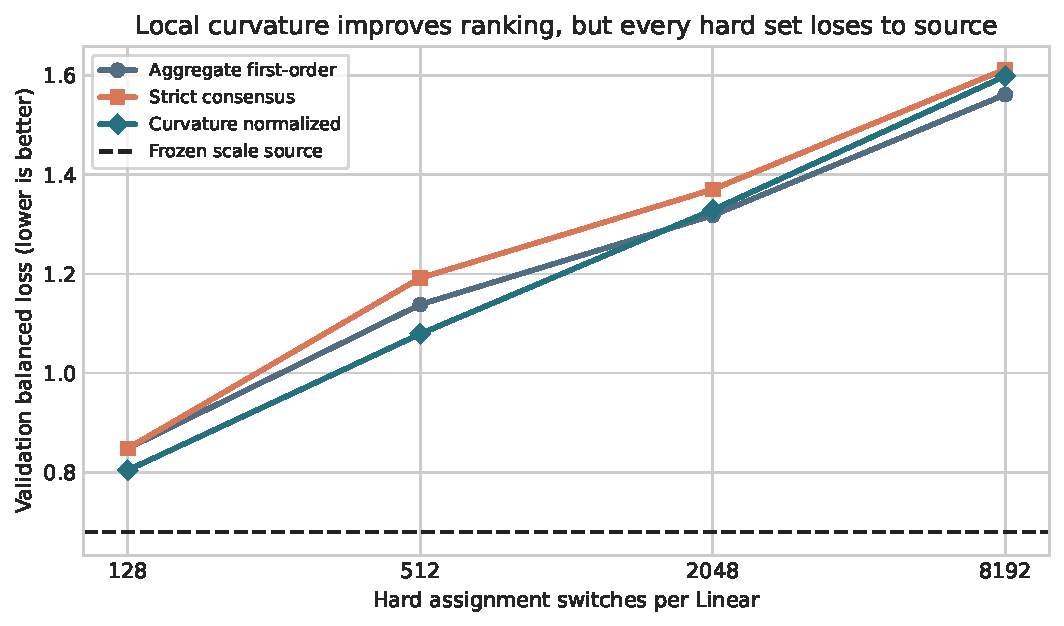
\includegraphics[width=\linewidth]{../img/v12_curvature_predictor.pdf}
\caption{曲率改善严格共识排序，但所有hard set都输给冻结scale source。}
\label{fig:v12}
\end{figure}

\begin{table}[t]
\centering
\small
\caption{Validation balanced loss（越低越好）。预算为每Linear切换数。}
\begin{tabular}{rrrr}
\toprule
预算 & Aggregate & Consensus & Curvature\\
\midrule
0/source & \multicolumn{3}{c}{\textbf{0.679691}}\\
128 & 0.848070 & 0.848267 & \textbf{0.804163}\\
512 & 1.138119 & 1.191663 & \textbf{1.078899}\\
2048 & \textbf{1.317897} & 1.370206 & 1.328956\\
8192 & \textbf{1.561233} & 1.612292 & 1.598649\\
\bottomrule
\end{tabular}
\end{table}

曲率对consensus为4/4胜，平均loss从1.255607降至1.202667；对aggregate只有2/4胜，未达到预注册3/4。最佳曲率集合为128/Linear，共3584个switch；Macro 70.8594\%，较source 76.3281\%低5.4688个百分点，loss 0.804163相对source恶化18.313\%。

\subsection{终态与机制}

Gate失败后候选audit未访问、checkpoint未写、完整assignment训练未授权、正式PPL/lm\_eval未运行。已有source指标只描述相同部署状态，不是V12新测量。

对集合$S$，$\mathcal L(W+\delta_S)=\mathcal L(W)+g^\top\delta_S+\frac12\delta_S^\top H(\xi)\delta_S$。逐候选$q_i$只近似部分对角项；$\delta_i^\top H\delta_j$与沿后续层传播的激活变化均被遗漏。曲率小预算更优而大预算失去优势，符合遗漏交叉项随集合增长累积的解释，但本文不声称已经单独估计这些项。

\subsection{局限与基线边界}

实验只覆盖一个8B模型最后四层，不能外推到所有架构。任务监督与QTIP等通用PTQ设置不同，本轮也没有新部署端点，因此不能声称超过QTIP或GSQ。负结果只否定当前8-way邻域、冻结scale锚点和局部对角曲率，不是否定所有assignment优化。
